\documentclass[../main.tex]{subfiles}

\begin{document}

\section{Meson mixing en oscillaties}%
\label{sec:meson_mixing_en_oscillaties}

\subsection{2-state systemen}%
\label{sub:2_state_systemen}

Meson mixing is niets meer dan gewone kwantummechanica. Als 2 toestanden dezelfde kwantumtoestanden binnen de behoudswetten zullen deze 2 toestanden opmengen met elkaar, in essentie zijn dit dezelfde toestanden. Hebben we $A$ en $B$ als 2 zo een toestanden dan krijgen we
\begin{equation}
    \begin{aligned}
        \label{eq:opmenhing_2_toestanden}
        A & \leftrightarrow B \\
        \left| \phi\right>&=c_{a}\left|\phi_{a}\right>+c_{b}\left| \phi_{b} \right>\\
        |\phi|^{2} &=\left|c_{a}\right|^{2}+\left|c_{b}\right|^{2}
    \end{aligned}
\end{equation}
Hierbij is de uiteindelijke golffunctie van deze 2 deeltjes een opmenging van de 2. De waarschijnlijkheden voor het ene of andere deeltje kunnen afhangen van de tijd en zullen dus oscileren. Een opmerking hierbij is dat bijvoorbeeld een elektron niet in een positron zal kunnen oscileren vanwege het behoud van lading. Voor de oscilatie tussen het proton en neutron is dit iets ingewikkelder. Alle krachten behalve de zwakke interactie behouden de isospin en zullen dus niet in elkaar oscileren. Dit is niet het geval bij de zwakke interactie die deze deeltjes met veel plezier zal laten overgaan. Zo is het alleen mogelijk dat deeltje/antideeltjes in elkaar kunnen overgezet worden waarbij behoud van massa lettend op overlappende breedtes ook behouden moet worden. Daarboven moet de lading ook behouden worden en houden we enkel neutrale toestanden over zoals neutrale mesonen en neutrinos.

\subsection{Meson mixing}%
\label{sub:meson_mixing}

Met de restricties hierboven opgenoemd zijn er nog maar een aantal mogelijke meson opmenginen mogelijk. Deze zijn:
\begin{equation}
    \begin{aligned}
        \label{eq:mogelijke_meson_opmengingen}
        \begin{array}{ll}
            \left|K^{0}\right>=\left| d \bar{s}\right> & \left|\bar{K}^{0}\right>=\left| \bar{d} s\right> \\
            \left|D^{0}\right>=\left| c \bar{u}\right> & \left|\bar{D}^{0}\right>=\left| \bar{c} u\right> \\
            \left|B_{d}^{0}\right>=\left| d \bar{b}\right> & \left|\bar{B}_{d}^{0}\right>=\left| \bar{d} b\right> \\
            \left|B_{s}^{0}\right>=\left| s \bar{b}\right> & \left|\bar{B}_{s}^{0}\right>=\left| \bar{s} b\right>
        \end{array}
    \end{aligned}
\end{equation}
De onderindex $d$ of $s$ bij het $B$ meson wijst op het hebben van een $d$ of $s$ quark. De reden waarom $\pi^0=\left|u\bar{u}\right>$ hier niet bij zit is omdat dit dezelfde hetzelfde zijn bij uitwisseling. Historisch zagen we dat $\bar{K}^{0}$ en $K^{0}$ vervallen in 2 en 3 pionen wat zou zeggen dat de pariteit van dit meson zowel $\pm1$ is.
\begin{equation}
    \begin{aligned}
        \label{eq:kaon_pion_verval}
            \bar{K}^{0} / K^{0} & \rightarrow & 2 \pi & & P=C P=+1 \\
                                & \rightarrow & 3 \pi & & P=C P=-1
    \end{aligned}
\end{equation}
Deze oscillaties gebeuren door 2 zwakke wisselwerkingen, $K^{0} \leftrightarrow(2 / 3) \pi \leftrightarrow \bar{K}^{0}$. Dit is het oude beeld dat we hiervan hebben.

\subsection{Box diagrammen}%
\label{sub:box_diagrammen}

Vandaag de dag weten we dat deze kaonen bestaan uit elk 2 quarks die aan de hand van $W$ bosonen zullen uitwisselen.

\begin{figure}[h]
    \centering
    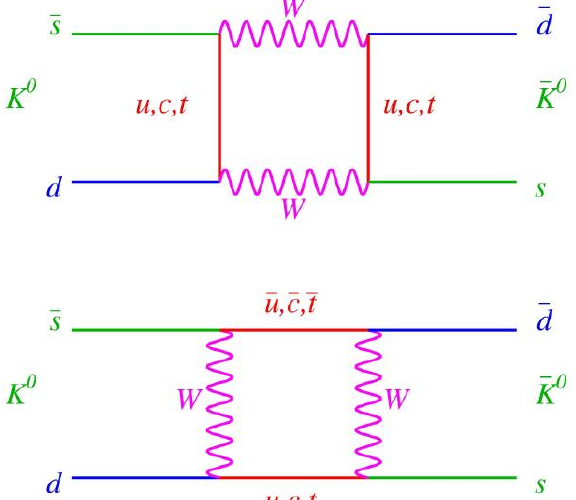
\includegraphics[width=0.4\linewidth]{meson_mixing_and_oscillations/box_diagrams.png}
    \caption{Box diagrammen van de kaon oscilaties}%
    \label{fig:meson_mixing_and_oscillations/box_diagrams}
\end{figure}

Zoals je kan zien is dit een 2de orde zwakke wisselwerkingen wat natuurlijk heel onwaarschijnlijk maar niet onmoglelijk is en de pariteit zal geschonden worden. Wat van groot belang is dat we intermediar naast de $W$ bosonen ook een een quark of antiquark zijn. We zijn hier dus met andere woorden gevoelig voor de koppeling tussen $d$ of $s$ en $u$, $c$ of $t$. Dit is iets waar we vandaag de dag nog veel onderzoek naar doen. Op dit moment gaan we er nog van uit dat de $CP$ pariteit behouden is.

\subsection{Mixen}%
\label{sub:mixen}

We gaan er hier van uit de $CP$ nog behouden is maar zien in dat $\bar{K}^{0}$ en $K^{0}$ niet de correcte eigentoestanden zijn omdat deze in elkaar worden omgezet.
\begin{equation}
    \begin{aligned}
        \label{eq:cp_anti_kaon}
        C P\left|K^{0}\right>=\left| \bar{K}^{0}\right>\quad C P\left|\bar{K}^{0}\right>=\left| K^{0}\right>
    \end{aligned}
\end{equation}
Het vervallen naar 2 verschillende hoeveelheden pionen is nu geen probleem meer omdat dit niet eens eigentoestanden zijn van $CP$ maar wel van $P$. Om correct te vervallen naar 2 of 3 pionen die $CP$ pariteit volgen moeten we ook voor de kaonen $CP$ eigentoestanden bepalen.
\begin{equation}
    \begin{aligned}
        \label{eq:kaon_cp_eigentoestanden}
        \left| K_{1}^{0}\right>&=\frac{1}{\sqrt{2}}\left[\left|K^{0}\right>+\left| \bar{K}^{0}\right>\right] & & C P=+1 \\
        \left| K_{2}^{0}\right>&=\frac{1}{\sqrt{2}}\left[\left|K^{0}\right>-\left| \bar{K}^{0}\right>\right] & & C P=-1
    \end{aligned}
\end{equation}
Dit kan ook nog herschreven worden tot
\begin{equation}
    \begin{aligned}
        \label{eq:kaon_cp_eig_mat}
        \left(\begin{array}{c}
            \left| K_{1}^{0}\right> \\
            \left| K_{2}^{0}\right>
            \end{array}\right)=\left(\begin{array}{cc}
                \cos \theta & \sin \theta \\
                -\sin \theta & \cos \theta
            \end{array}\right)\left(\begin{array}{c}
            \left| \bar{K}^{0}\right> \\
            \left| K^{0}\right>
        \end{array}\right)\\
        \left(\begin{array}{c}
            \left| m_{1}\right> \\
            \left| m_{2}\right>
            \end{array}\right)=\left(\begin{array}{cc}
                \cos \theta & \sin \theta \\
                -\sin \theta & \cos \theta
            \end{array}\right)\left(\begin{array}{c}
            \left| s_{1}\right> \\
            \left| s_{2}\right>
        \end{array}\right)
    \end{aligned}
\end{equation}
Dit zal dus een relatie geven tussen de massa eigentoestanden die vrij kunnen rond bewegen en de symmetrie eigentoestanden met definiete strangeness. In dit geval is de $\theta=45^\circ$. In essentie zijn de $s$ eigentoestanden van de sterke wisselwerking die de kaonen maakt en de $m$ eigentoestanden van de zwakke wisselwerking die zullen vervallen naar de pionen.\\
Hierbij moet de $CPT$ nog steeds behouden zijn wat wil zeggen dat $m(part) = m(\bar{part})$ of de $m(K^0) = m(\bar{K}^0)$ moet zijn. Maar de $\left|\bar{K}_{1}^{0}\right>\neq\left| K_{2}^{0}\right>$ en dat de massas niet perse gelijk moeten zijn aan elkaar. De massa van het kaon zal dus afhangen van hoe we er naar kijken, met de zwakke of sterke wisselwerking.

\subsection{Oscillaties}%
\label{sub:oscillaties}

Tijdens de oscillatie zal de massa eigentoestand propageren: $m_{i}(t)=m_{i}(0) e^{-i\left(m_{i}-i \frac{\Gamma_{i}}{2}\right) t}$. Hierbij wordt verondersteld dat de kaonen stil staan en een massa hebben. De 2de term in de exponent geeft de vervalsnelheid van de massatoestanden naar pionen terug.\\
Bekijken we nu het voorbeeld waar op tijdstip $t=0$ een pure $s_2$ toestand wordt waargenomen. Dit komt overeen met $s_{1}(0)=0, s_{2}(0)=1$. Indien we deze toestanden nu stabiel beschouwen hebben we $\Gamma_i = 0$ en krijgen we voor de massa toestanden:
\begin{equation}
    \begin{aligned}
        \label{eq:voorbeeld_osc_stable_massa}
        s_{1}(0)=m_{1}(0) \cos \theta-m_{2}(0) \sin \theta=0 \\
        s_{2}(0)=m_{1}(0) \sin \theta+m_{2}(0) \cos \theta=1
    \end{aligned}
\end{equation}
Om aan dit stelsel te voldoen moet $m_1(0) = \sin\theta$ en $m_2(0) = \cos\theta$ zijn. Vullen we de tijd propagatie door dan krijgen we 
\begin{equation}
    \begin{aligned}
        \label{eq:voorbeeld_osc_stable_massa_tijd_prop_1}
        s_{1}(t) &=m_{1}(t) \cos \theta-m_{2}(t) \sin \theta \\
                 &=\sin \theta \cos \theta\left[e^{-i m_{1} t}-e^{-i m_{2} t}\right] \\
                 &=\frac{\sin (2 \theta)}{2} e^{-\frac{i\left(m_{1}+m_{2}\right) t}{2}}\left[e^{-\frac{i\left(m_{1}-m_{2}\right) t}{2}}-e^{-\frac{i\left(m_{2}-m_{1}\right) t}{2}}\right]
    \end{aligned}
\end{equation}
De reden voor het herschrijven naar de uitgebreide vorm is omdat we nu mooie oscillatietermen krijgen die we kunnen herschrijven naar sinussen ($\sin (\theta) = \frac{1}{2 i}\left(e^{+i \theta}-e^{-i \theta}\right)$).
\begin{equation}
    \begin{aligned}
        \label{eq:voorbeeld_osc_stable_massa_tijd_prop_2}
        s_{1}(t)=\frac{\sin (2 \theta)}{2}(2 i) \sin \left(\frac{\Delta m \cdot t}{2}\right) e^{-\frac{i\left(m_{1}+m_{2}\right) t}{2}}
    \end{aligned}
\end{equation}
Zo kan je zien dat er een oscilatie volgens de tijd zal komen inkruipen in deze uitwerking. De waarschijnlijkheid om $s_1$ te vinden wordt gegeven door:
\begin{equation}
    \begin{aligned}
        \label{eq:voorbeeld_osc_stable_massa_prob_1}
        P\left(s_{1}\right)=\left|s_{1}(t)\right|^{2}=\sin ^{2}(2 \theta) \sin ^{2}\left(\frac{\Delta m \cdot t}{2}\right)
    \end{aligned}
\end{equation}
Door het kwadrateren van $s_1$ zal de exponentiële factor weg vallen. Belangrijk om te zien is dat de amplitude bepaald wordt door $\theta$ met een maximale waarde bij $\sin^2(2\theta)=1 \rightarrow \theta=45^\circ$ en deat de periode bepaald wordt door $\Delta m$.
\begin{equation}
    \begin{aligned}
        \label{eq:voorbeeld_osc_stable_massa_prob_2}
        P\left(s_{2}\right)=1-\left|s_{1}(t)\right|^{2}=1-\sin ^{2}(2 \theta) \sin ^{2}\left(\frac{\Delta m \cdot t}{2}\right)
    \end{aligned}
\end{equation}

\subsection{$K^0$-systeem}%
\label{sub:_k_0_systeem}

Nu we weten hoe de waarschijnlijkheid er uit ziet voor deeltjes die niet vervallen kunnen we het onszelf iets moeilijker maken door de kaonen ook te laten vervallen. Kijken we naar de massatoestanden van het kaon die zo goed als dezelfde massa hebben.\\
\begin{minipage}[c]{0.5\textwidth}
    \begin{center}
        $\left| K_1 \right> \rightarrow 2\pi$
    \end{center}
    \begin{itemize}
        \item Omdat deze maar vervalt in 2 pionen is er nog veel faseruimte over (een factor $p^2 dp$ aanwezig).
        \item Wordt waargenomen als $\left| K_S^0 \right>$
        \item Omdat deze veel faseruimte over heeft zal hij ook snel vervallen.
            \begin{equation}
                \begin{aligned}
                    \label{eq:verval_ks}
                    \tau_{S}&=(8.954 \pm 0.004) \cdot 10^{-11} \text{s}\\
                    \Gamma_S &= 7.4\mu\text{eV}\\
                    c\tau_S &= 2.6844\text{cm}
                \end{aligned}
            \end{equation}
    \end{itemize}
\end{minipage}\noindent
\begin{minipage}[c]{0.5\textwidth}
    \begin{center}
        $\left| K_2 \right> \rightarrow 3\pi$
    \end{center}
    \begin{itemize}
        \item Deze heeft niet veel faseruimte over
        \item Wordt waargenomen als $\left| K_L^0 \right>$
        \item Omdat deze weinig faseruimte over heeft zal hij ook langer leven.
            \begin{equation}
                \begin{aligned}
                    \label{eq:verval_ks}
                    \tau_{L}&=(5.116 \pm 0.021) \cdot 10^{-8} \text{s}\\
                    \Gamma_L &= 0.013\mu\text{eV}\\
                    c\tau_L &= 15.34\text{m}
                \end{aligned}
            \end{equation}
    \end{itemize}
\end{minipage}
Met deze informatie bekijken we nu de het voorbeeld waar bij $t=0$ het systeem zich in een pure $\left| K^0 \right>$ toestand bestaat. Dit wilt dus zeggen dat $K^0(0) = 1$ en $\bar{K}^0 = 0$ of $K_1(0)=K_2(0)= \frac{1}{\sqrt{2}} $. Propageren we deze toestanden nu door de tijd dan krijgen we op tijdstip $t$:
\begin{equation}
    \begin{aligned}
        \label{eq:voorbeeld_kaon_osc_tijd_prop_1}
        K^{0}(t) &=\frac{1}{\sqrt{2}}\left(K_{1}(t)+K_{2}(t)\right) \\
        \bar{K}^{0}(t) &=\frac{1}{\sqrt{2}}\left(K_{1}(t)-K_{2}(t)\right)
    \end{aligned}
\end{equation}
Vullen we hier de propagatie van de massatermen uit de vorige sectie in dan krijgen we:
\begin{equation}
    \begin{aligned}
        \label{eq:voorbeeld_kaon_osc_tijd_prop_2}
        K^{0}(t) &=\frac{1}{2}\left(e^{-i m_{1} t-\frac{\Gamma_{1}}{2} t}+e^{-i m_{2} t-\frac{\Gamma_{2}}{2} t}\right) \\
        \bar{K}^{0}(t) &=\frac{1}{2}\left(e^{-i m_{1} t-\frac{\Gamma_{1}}{2} t}-e^{-i m_{2} t-\frac{\Gamma_{2}}{2} t}\right)
    \end{aligned}
\end{equation}
Het verschil met vorige sectie \ref{sub:oscillaties} is nu dat de vervaltermen in de exponenten aanwezig zijn. Dit zal de berekening van de de probabiliteiten wel iets moeilijker maken. De waarschijnlijkheid dat we overgaan van een $K^0$ naar een $\bar{K}^0$ kan als volgt uitgewerkt worden.
\begin{equation}
    \begin{aligned}
        \label{eq:voorbeeld_kaon_osc_tijd_prop_3}
        P\left(K^{0} \rightarrow \bar{K}^{0}\right) &=\left|\bar{K}^{0}(t) \bar{K}^{0 *}(t)\right| \\
                                                    &=\frac{1}{4}\left(e^{-\Gamma_{1} t}+e^{-\Gamma_{2} t}-e^{+i \Delta m t} e^{-\Gamma t}-e^{-i \Delta m t} e^{-\Gamma t}\right) \\
                                                    &=\frac{1}{4}\left(e^{-\Gamma_{1} t}+e^{-\Gamma_{2} t}-2 \cos (\Delta m t) e^{-\Gamma t}\right)
    \end{aligned}
\end{equation}
Hierbij is $\Gamma = \frac{\Gamma_1 \Gamma_2}{2}$. Om van $K_0$ naar $K_0$ is nu makkelijk te vinden.
\begin{equation}
    \begin{aligned}
        \label{eq:voorbeeld_kaon_osc_tijd_prop_4}
        P\left(K^{0} \rightarrow K^{0}\right) &= 1-P\left(K^{0} \rightarrow \bar{K}^{0}\right)\\
                                              &=\frac{1}{4}\left(e^{-\Gamma_{1} t}+e^{-\Gamma_{2} t}+2 \cos (\Delta m t) e^{-\Gamma t}\right)
    \end{aligned}
\end{equation}
De waarschijnlijkheid dat er nog iets over is in het kaon systeem na tijd $t$ is
\begin{equation}
    \begin{aligned}
        \label{eq:voorbeeld_kaon_osc_tijd_prop_5}
        P\left(K^{0} \rightarrow \bar{K}^{0}\right)+P\left(K^{0} \rightarrow K^{0}\right)=\frac{1}{2}\left(e^{-\Gamma_{1} t}+e^{-\Gamma_{2} t}\right)
    \end{aligned}
\end{equation}
In figuur \ref{fig:meson_mixing_and_oscillations/kaon_osc_tijd_plot} worden een aantal waarschijnlijkheden geplot in de functie van de tijd onder bepaalde condities.

\begin{figure}[h]
    \centering
    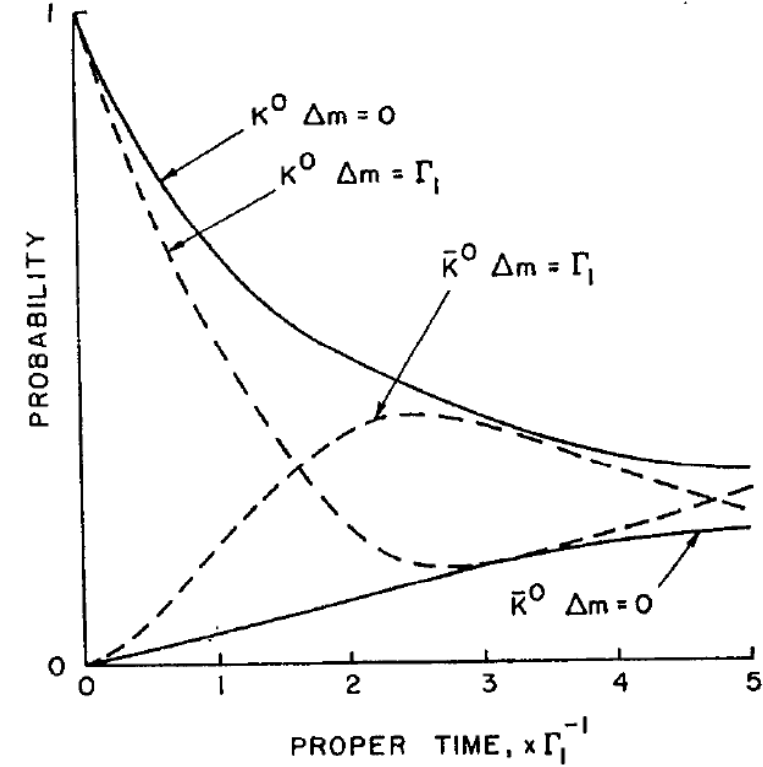
\includegraphics[width=0.5\linewidth]{meson_mixing_and_oscillations/kaon_osc_tijd_plot.png}
    \caption{Plot van kaon waarschijnlijkheden tijdens oscilaties}%
    \label{fig:meson_mixing_and_oscillations/kaon_osc_tijd_plot}
\end{figure}

Ten eerste als we kijken naar het geval dat de massa van de kaonen gelijk zijn ($\Delta m = 0$) valt de $\cos(\Delta m t)$ weg uit de vergelijkingen en kwasi exponentieel verval voor $K_0$. In het begin van de oscillaties wordt het verval geleid door $\Gamma_1$ en later door $\Gamma_2$. Indien $\Delta m$ verschillend van 0 is dan zal het meest waarschijnlijke deeltje afwisselen in de tijd waarbij de amplitude tussen de probabiliteiten afneemt in de tijd.\\
De belangrijkste puntjes dat we hier moeten onthouden zijn:
\begin{itemize}
    \item De kaonen oscileren enkel als $\Delta m \neq 0$.
    \item Het exponentiële verval wordt gedomineerd door de kortste levensduur. Voor het Kaon systeem is dit $K_S$.
\end{itemize}

\subsection{Experiment}%
\label{sub:experiment}

Hoe is het nu mogelijk om een onderscheid te maken tussen $K^0$ en $\bar{K}^0$?\\
Kijken we naar deze kaonen met de sterke interactie dan zien we het volgende:
\begin{equation}
    \begin{aligned}
        \label{eq:kaon_sterke_int}
        \bar{K}^{0}+p &\rightarrow & \pi^{+}+\Lambda \\
        \bar{d} s+u u d & &\rightarrow u \bar{d}+u d s \\
        K^{0}+p & &\centernot\rightarrow \pi^{+}+\Lambda \\
        d \bar{s}+u u d & &\centernot\rightarrow u \bar{d}+u d s
    \end{aligned}
\end{equation}
Als we kijken naar de quarks van de kaonen en het proton zal het voor $K^0$ niet mogelijk zal zijn om $\bar{s}$ door te geven om een $\Lambda$ te maken. $K^0$ zal dus zo goed als niet interageren met het proton.\\
Aan de hand van de zwakke interactie is het ook mogelijk om het verschil tussen de kaonen aan te voelen. Het zal altijd de $s$ quark of antiquark zijn die via een $W^\pm$ boson zal vervallen naar een $u$ quark of antiquark.

\begin{figure}[h]
    \centering
    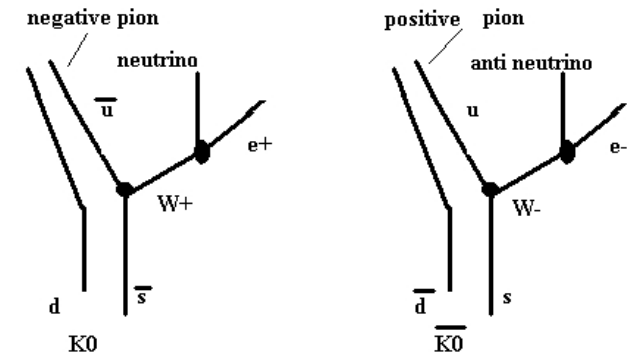
\includegraphics[width=0.4\linewidth]{meson_mixing_and_oscillations/kaon_zwak_verval.png}
    \caption{Feynman diagrammen van het zwak verval van kaonen}%
    \label{fig:meson_mixing_and_oscillations/kaon_zwak_verval}
\end{figure}

Hierdoor krijgen we verschillende einddeeltjes die in experimenten makkelijk uit elkaar te houden zijn.
\begin{equation}
    \begin{aligned}
        \label{eq:kaon_zwak_verval}
        \bar{K}^{0} &\rightarrow \pi^{+}+e^{-}+\bar{\nu}_{e} \\
        K^{0} &\rightarrow \pi^{-}+e^{+}+\nu_{e}
    \end{aligned}
\end{equation}
Het verval van het $W$ boson kan natuurlijk ook hadronisch gebeuren en krijgen we 2 keer dezelfde uiteindelijke toestand $\pi^+\pi^-$. Bij het verval naar leptonen hebben we niet een bepaalde $CP$ net zoals bij de kaon toestanden.\\
Wat gebeurt er nu juist. We maken aan de hand van de sterke interactie een zuivere $\left|K^0\right>=\left|\bar{d}s\right>$ toestand aan. Het vervallen van deze toestand is enkel mogelijk via de zwakke interactie op een semi leptonische manier (veglijking (\ref{eq:kaon_zwak_verval})) of op een hadronische manier. Hierbij wordt er ofwel vervallen via de $K^0$ en $\bar{K}^0$ componenten of van de $K_1$ en $K_2$ componenten.\\
Het is dus mogelijk aan de hand van assymetrie van de lading van de uitkomende leptonen te weten wat de ratio aan $K^0/\bar{K}^0$ te taggen.
\begin{equation}
    \begin{aligned}
        \label{eq:lepton_lading_assymetrie}
        A=\frac{N_{+}-N_{-}}{N_{+}+N_{-}}
    \end{aligned}
\end{equation}
Deze $A$ zal tussen -1 en 1 varieren met 1 die overeen komt met $t=0$ en 0 als er even veel $K^0$ en $\bar{K}^0$ aanwezig zijn. Deze oscillaties zijn mooi gemeten in experimenten.

\begin{figure}[h]
    \centering
    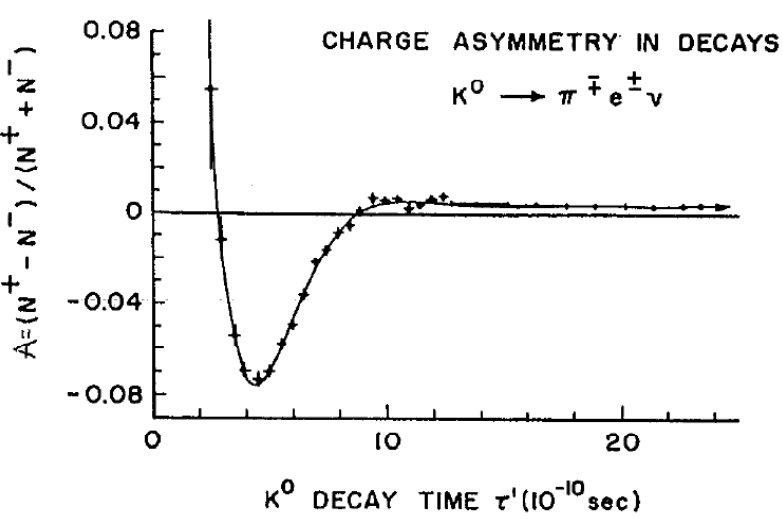
\includegraphics[width=0.5\linewidth]{meson_mixing_and_oscillations/kaon_osc_verval.png}
    \caption{Assymetrie onderzoek van de kaon oscilaties}%
    \label{fig:meson_mixing_and_oscillations/kaon_osc_verval}
\end{figure}

Dit gaat over heel kleine tijden. met een sterk gedempte oscilatie. Uit deze demping kunnen we het massaverschil bepalen $\Delta m=(0.5293 \pm 0.0009) \times 10^{-10} \text{s}^{-1} = (3.484 \pm 0.006) \times 10^{-12} \text{MeV}$. De reden waarom dit niet volledig naar 0 gaat is door $CP$ schending waar we later op verder gaan.

\subsection{Regeneratie}%
\label{sub:regeneratie}

Vertrekken we met een bundel kaonen $K^0$ of $\bar{K}^0$. Die zullen direct beginnen vervallen in pionen waarbij de $K_S$ met een weglengte van 3cm na 10cm allemaal vervallen zijn naar 2 pionen. We hebben dus alleen nog maar $K_L$ over. Plaatsen we in deze bundel nu een bulk materiaal. Kaonen zijn ongeladen deeltjes dus zullen ze makkelijk door het materiaal bewegen. In het materiaal zullen de kaonen sterk interageren met de nucleonen (nucleaire reacties). Na de botsing kunnen we terug spreken over $K^0$ en $\bar{K}^0$ omdat deze sterke wisselwerking ondergaan zijn. Er zullen naast $K_L$ ook terug $K_S$ aanwezig zijn. We hebben ze als het ware geregenereerd. Dit gaat als volgt:
\begin{equation}
    \begin{aligned}
        \label{eq:ks_regen}
        K_{L}=K_{2}&=\frac{1}{\sqrt{2}}\left(K^{0}-\bar{K}^{0}\right)\\
        \rightarrow \frac{1}{\sqrt{2}}\left(f K^{0}-\bar{f} \bar{K}^{0}\right)&=\frac{1}{2}\left(f\left(K_{S}+K_{L}\right)-\bar{f}\left(K_{S}-K_{L}\right)\right) \\
                                                                              &=\frac{1}{2}\left((f-\bar{f}) K_{S}+(f+\bar{f}) K_{L}\right)
    \end{aligned}
\end{equation}
In het geval dat $f\neq \bar{f}$ zien we dat $K_S$ zal geregenereerd worden. Kijken we alleen al naar de interactie van de kaonen met het proton (vergelijking (\ref{eq:kaon_sterke_int})) vergelijken zien we al direct dat $f$ groter zal zijn dan $\bar{f}$.

\subsection{Tijd afhankelijkheid}%
\label{sub:tijd_afhankelijkheid}

We hebben al gezien dat de tijd afhankelijkheid bepaald wordt door $\Delta m$. Integreren we dit over de tijd kunnen we zien wat de waarschijnlijkheid was om van $K^0$ naar $\bar{K}^0$ te gaan in vergelijking tot de totale oscillaties.
\begin{equation}
    \begin{aligned}
        \label{eq:kaon_osc_tijd_int}
        \chi=\frac{\int_{0}^{\infty} P\left(K^{0} \rightarrow \bar{K}^{0}\right) d t}{\int_{0}^{\infty}\left(P\left(K^{0} \rightarrow \bar{K}^{0}\right)+P\left(K^{0} \rightarrow K^{0}\right)\right) d t}=\frac{1}{2} \frac{x^{2}+y^{2}}{1+x^{2}}
    \end{aligned}
\end{equation}
met $x= \frac{\Delta m}{\Gamma}$ en $y= \frac{\Delta \Gamma}{2\Gamma} = \frac{\Gamma_L-\Gamma_S}{\Gamma_L + \Gamma_S}$. Hierbij zal $0\leq \chi \leq 0.5$ variëren. {\color{blue} Ryckbosch zegt dat het een goed idee is om deze integralen eens uit te rekenen maar zegt letterlijk dat dit geen examen leerstof is.} Deze verlijking zal iets zeggen over de opmenging. De $x$ zegt ons dat er enkel opmenging zal zijn als $\Delta m$ en $\Gamma$ van dezelfde orde moeten zijn.

\subsection{Kaon systeem resultaten}%
\label{sub:kaon_systeem_resultaten}

We zitten hier naar een effect te kijken van $\Delta m_K = (3.483 \pm 0.006) \times 10^{-6} \text{eV}$ tegenover de massa $m_K = 450$MeV. Dit betekent dat we kijken naar een effect $\sim O(10^{-15}$ kleiner dan de zijn massa nog steeds mooi zichtbaar is. De verval breedte van dit systeem komt overeen met $\Gamma=\frac{\Gamma_{S}+\Gamma_{L}}{2} \approx \frac{\Gamma_{S}}{2}=3.7 \times 10^{-6} \text{eV}$. Hier is het duidelijk dat $x$ ongeveer 1 zal zijn en de oscillatie zal doorgaan.
\begin{equation}
    \begin{aligned}
        \label{eq:kaon_osc_exp_results}
        x_{K} &=0.94 \\
        y_{K} &=0.998 \\
        \chi_{K} &=0.499
    \end{aligned}
\end{equation}
$x$ vertelt ons hoeveel oscillaties we krijgen per levensduur wat in dit geval dus 1 is.

\subsection{$B$-meson systeem}%
\label{sub:_b_meson_systeem}

Het kaon systeem is een beetje van een uitzondering op het vlak van het aantal verval kanalen. Deze heeft er veel minder dan de andere mesonen waardoor $y$ veel groter is dan bij de andere meson waar $y$ eerder 0 zal zijn.\\
Kijken we naar de $B$ mesonen die zwaar zijn ($\approx 5.3$GeV). Dit wil zeggen dat er veel verval kanalen zijn en $\tau \approx 1.5$ps of $c\tau \approx 450\mu$m. Om dit probleem van de korte levensduur te ontwijken geven we ze een Lorentz boost. In dit geval kunnen ze een afstand $d=\gamma\beta c\tau$ afleggen. Het aanmaken van $B$ mesonen kan op verschillende manieren gedaan worden. In LEP werd dit gedaan aan de hand van $Z$ bosonen, $e^{+} e^{-} \rightarrow Z^{0} \rightarrow b \bar{b} \rightarrow B^{0} \bar{B}^{0}$. Met een massa van het $Z$ boson rond de $90$GeV hebben de $b$ quarks ongeveer $45$GeV aan energie hebben. Een andere manier is de asymmetrische B-factories ($e^{+} e^{-} \rightarrow \Upsilon(4 S) \rightarrow B^{0} \bar{B}^{0}$). Het verschil in energie tussen de initiële elektronen en positronen zal een boost geven aan de $B$ mesonen. De $B$ oscillaties zijn voor het eerste waargenomen in 1986 in het ARGUS experiment waar het volgende verval is waargenomen: $e^{+} e^{-} \rightarrow \Upsilon \rightarrow B^{0} \bar{B}^{0} \rightarrow B^{0} B^{0}$.

\begin{figure}[h]
    \centering
    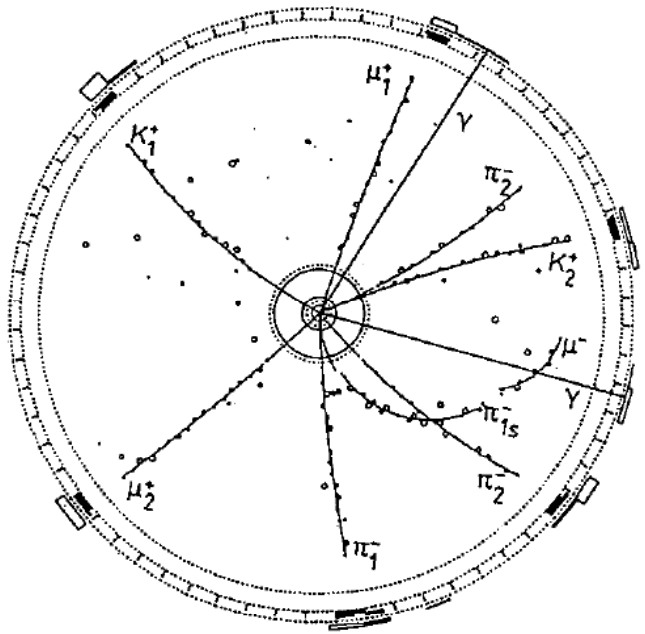
\includegraphics[width=0.4\linewidth]{meson_mixing_and_oscillations/argus.png}
    \caption{ARGUS experiment}%
    \label{fig:meson_mixing_and_oscillations/argus}
\end{figure}

In de resultaten die we hier zien in het ARGUS experiment zit heel veel informatie. We kunnen in de tracking kamer veel deeltjes waarnamen maar niet in de $B$ mesonen. Deze worden pas gedetecteerd in de calorimeter. Wat hier mooi is, is dat we geen $B^0$ en $\bar{B}^0$ waarnemen maar eerder 2 $B^0$. Dit is interessant om te bekijken. Er zijn 2 vervallen die zullen gebeuren.
\begin{equation}
    \begin{aligned}
        \label{eq:argus_vervallen}
        B_{1}^{0} \rightarrow & D_{1}^{*-} \mu_{1}^{+} \nu_{1} \\
                              & D_{1}^{*-} \rightarrow \pi_{1}^{-} \bar{D}^{0} \\
                              & \bar{D}^{0} \rightarrow K_{1}^{+} \pi_{1}^{-} \\
        B_{2}^{0} \rightarrow & D_{2}^{*-} \mu_{2}^{+} \nu_{2} \\
                              & D_{2}^{*-} \rightarrow \pi^{0} D^{-} \\
                              & D^{-} \rightarrow K_{2}^{+} \pi_{2}^{-} \pi_{2}^{-}
    \end{aligned}
\end{equation}
Voor beide gevallen hebben we een $B^0=d\bar{b}$ waarbij de $b$ antiquark zal vervallen aan de hand van de zwakke interactie die een $W$ boson geven ($\bar{b} \rightarrow \bar{c}+W^{+}$) dat zal vervallen in een muon en een neutrino. Voor $B_1^0$ krijgen we uiteindelijk 5 uitgaande deeltjes $\mu_1^+$, $\nu_1$, $\pi_1^-$, $K_1^+$ en $\pi_1^-$ waarbij de neutrino natuurlijk niet gedetecteerd wordt. Het pion dat wordt aangemaakt bij het verval van het geëxiteerde $D^{*-}$ meson is laag energetisch omdat er bijna geen verschil is tussen de massa van het geëxiteerde $D$ meson en bij de grondtoestand ($2010\text{GeV}\rightarrow1865$GeV).
\begin{equation}
    \begin{aligned}
        \label{eq:argus_verval_1}
        B^0     &                   & 5280\text{GeV}    \\
                & \downarrow \mu    &                   \\
        D^{*0}  &                   & 2010\text{GeV}    \\
                & {\color{red} \downarrow \pi_s}    &   \\
        D^0     &                   & 1865\text{GeV}    \\
                & \downarrow \mu    &                   \\
        K^+     &                   & 494\text{GeV}     \\
    \end{aligned}
\end{equation}
Dit kan ook gezien worden in figuur \ref{fig:meson_mixing_and_oscillations/argus} waar we 1 pion kunnen zien dat een veel meer afbuigt dan de rest. Dit is het pion met lage snelheid. Omdat we al een $B^0$ hebben zouden we verwachten dat het tweede $B$ boson $\bar{B}$ zou zijn en we dus een $\mu^-$ zouden waarnemen. Dit zien we in het experiment niet want $\mu_2$ beweegt hier nog steeds in wijzers zin en is dus ook positief geladen. In dit geval krijgen we 6 uitgaande deeltjes $\mu_2^+$, $\nu_2$, $\pi^0$, $K_2^+$ en 2 keer $\pi_2^-$. Het neutrino wordt terug niet waargenomen en het $\pi^0$ zien we als 2 fotonen. Het belangrijke is hier toch het feit dat beide $B$ mesonen aan de hand van een $W^+$ boson. Dit wilt dus zeggen dat $\bar{B}^0$ zo snel is geoscilleerd naar $B^0$ dat het zelf geen tijd heeft gehad om te vervallen.

\subsection{Box diagrammen voor B mesonen}%
\label{sub:box_diagrammen_voor_b_mesonen}

\begin{figure}[h]
    \centering
    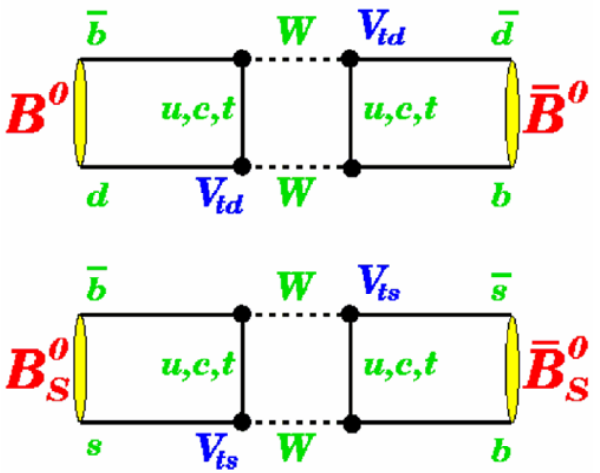
\includegraphics[width=0.5\linewidth]{meson_mixing_and_oscillations/box_diagr_b.png}
    \caption{Box diagrammen van de $B$ mesonen}%
    \label{fig:meson_mixing_and_oscillations/box_diagr_b}
\end{figure}

De reden waarom we vooral kijken naar $V_{td}$ en $V_{ts}$ is omdat de bottom quark zo goed als altijd aan de top quark zal binden. Deze box diagrammen zijn van hoog belang om te meten omdat dit de enige manier zijn om de elementen van de CKM-matrix te bepalen.

\subsection{Experimentele methodes voor B mesonen}%
\label{sub:experimentele_methodes_voor_b_mesonen}

Experimenteel  gaan we op dezelfde manier te werk als bij de $K$ mesonen (sectie \ref{sub:experiment}). De vervalkanalen die we bekijken zijn $B^{0} \rightarrow l^{+} \nu X$ en $\bar{B}^{0} \rightarrow l^{-} \bar{\nu} X$ waar $X$ eender welk ander deeltje kan zijn zoals bijvoorbeeld een $D$ meson. Deze $B$ mesonen zijn zwaar en vervallen snel. Omdat het voor allebei de vervallen zo kort is kan je geen onderscheid maken tussen long of short. Het onderscheid zal hier gemaakt worden aan de hand van de massa met $H$ voor heavy en $L$ voor light. Hierbij hebben we nog steeds dat $\Delta m = m_H - m_L > 0$. We verwachten ook dat $y = \frac{\Delta \Gamma}{2 \Gamma} \ll 1$. De eerste goede metingen van de oscillatie zelf zijn gedaan in OPAL.

\begin{figure}[h]
    \centering
    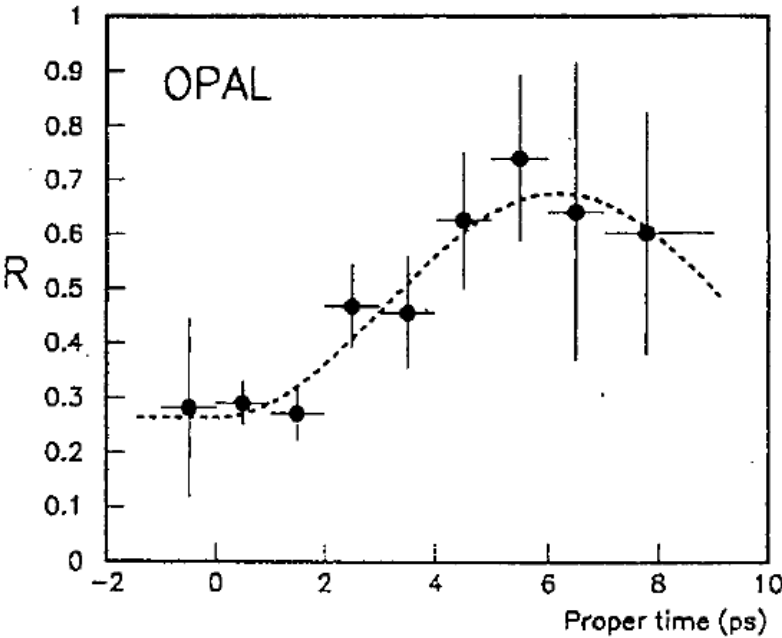
\includegraphics[width=0.6\linewidth]{meson_mixing_and_oscillations/b_osc_exp.png}
    \caption{OPAL onderzoek naar $B$ meson oscillaties}%
    \label{fig:meson_mixing_and_oscillations/b_osc_exp}
\end{figure}

Hier zien we de asymmetrie van deze deeltjes uitgezet in functie van de eigentijd van de $B$ mesonen. Na 1 oscillatie kunnen zien dat de foutenvlaggen heel groot worden. De mesonen zullen dus vervallen zijn.

\subsection{$B$-oscillaties resultaten}%
\label{sub:_b_oscillaties_resultaten}

Voor het $B$ meson met een $d$ quark hebben we:
\begin{equation}
    \begin{aligned}
        \label{eq:b_d_resultaten}
        \Delta m_{d} &=(3.337 \pm 0.033) \times 10^{-4} \text{eV} \\
        \Delta m_{d} &=(0.507 \pm 0.004) \times 10^{12} \text{s}^{-1}\\
        x_{d}&=0.770 \pm 0.008 \\
        \chi_{d}&=0.1862 \pm 0.0023
    \end{aligned}
\end{equation}
Voor $B$ mesonen met een $s$ quark is dit een stuk moeilijker en zijn deze resultaten maar in 2006 gevonden.
\begin{equation}
    \begin{aligned}
        \label{eq:b_s_resultaten}
        \Delta m_{s}&=(116.4 \pm 0.5) \times 10^{-4} \text{eV} \\
        \Delta m_{s}&=(17.69 \pm 0.08) \times 10^{12} \text{s}^{-1}\\
        x_{s}&=26.49 \pm 0.29 \\
        \chi_{s}&=0.499292 \pm 0.000016
    \end{aligned}
\end{equation}
Voor $B_S^0$ hebben we experimenteel gevonden dat deze 26 keer oscilleert voor hij vervalt.

\begin{figure}[h]
    \centering
    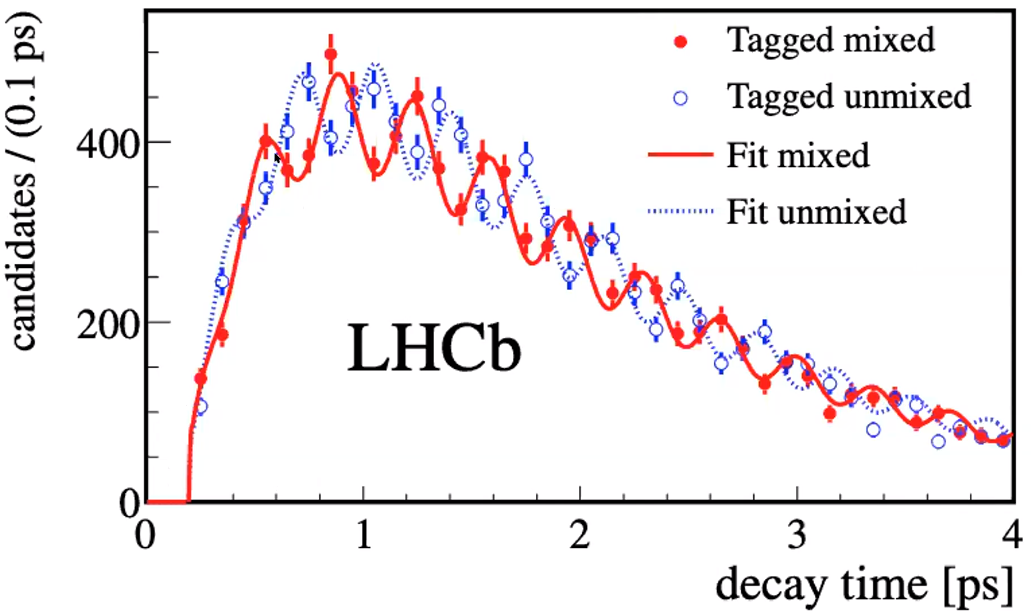
\includegraphics[width=0.5\linewidth]{meson_mixing_and_oscillations/b_s_osc_res.png}
    \caption{Huidige resultaten van de experimenten van $B_S$ oscillaties}%
    \label{fig:meson_mixing_and_oscillations/b_s_osc_res}
\end{figure}

Het belangrijkste in deze grafiek is dat er zo veel oscillaties gebeuren. Wat mixed en unmixed betekent is niet echt belangrijk. Regeneratie zal niet mogelijk zijn omdat zowel $B_H$ als $B_L$ ongeveer op hetzelfde moment zullen vervallen en krijgen we dus geen zuivere bundel van één van de 2 en is het niet mogelijk om het andere te regenereren.  Je zou hier denken dat deze toestanden makkelijk in elkaar kunnen oscilleren wegens de grote hoeveelheid oscillaties voor ze vervallen maar dit is niet correct. Het gemak van oscilleren wordt bepaald door de amplitude, niet de frequentie. De frequentie leidt terug naar dat massaverschil en wil dus zeggen dat we zitten te kijken naar de heel kleine overlap in de staarten van deze mesonen. Het zal dus juist heel onwaarschijnlijk zijn om deze oscillaties tegen te komen.

\subsection{$D$-oscillaties}%
\label{sub:_d_oscillaties}

$D$ mesonen zijn de enige mesonen waar een up quark aanwezig zal zijn.
\begin{equation}
    \begin{aligned}
        \label{eq:d_mes_osc}
        D^{0} &\leftrightarrow \bar{D}^{0}\\
        c \bar{u} &\leftrightarrow \bar{c} u
    \end{aligned}
\end{equation}
Dit is extreem moeilijk om waar te nemen omdat $\Delta m \ll \Gamma$ en met als gevolg dat $x\ll 1$. De reden voor het heel brede verval kanaal is omdat de $c$ quark binnen zijn doublet vervalt wat veel makkelijker is dan vervallen van de 3de naar 2de generatie voor de $K$ en $B$ mesonen. Het zal dus vervallen voor dat het zal oscilleren. Het is voor het eerst waargenomen in de 2013 waar ze keken naar
\begin{equation}
    \begin{aligned}
        \label{eq:ratio_d_osc}
        R=\frac{\sigma\left(D^{0} \rightarrow K^{+} \pi^{-}\right)}{\sigma\left(D^{0} \rightarrow K^{-} \pi^{+}\right)}
    \end{aligned}
\end{equation}
De cross sectie van de teller is deze van het geoscilleerd meson ($D^0 = \bar{c}u \rightarrow \bar{s}u+W^+ \rightarrow K^+\pi^-$). Hoe zijn we nu zo zeker dat we begonnen waren met $D^0$ en niet $\bar{D}^0$. Dit zijn we niet zeker. Het moment dat ze aangemaakt worden weten we alleen dat $R=0$ is omdat er even veel $c$ als $\bar{c}$'s worden aangemaakt. We hebben waargenomen aan LHC dat er over een bepaalde tijd meer kans is om een $\bar{c}u$ te zien vervallen dan $c\bar{u}$.

\subsection{Meson oscillaties}%
\label{sub:meson_oscillaties}

De reden om deze oscillaties te onderzoeken hebben we al aangehaald on sectie \ref{sub:box_diagrammen_voor_b_mesonen}. We willen de matrix elementen van de CKM matrix bepalen. Hoeveel van alle virtuele quarks aanwezig zal zijn hangt af van de hoeveelheid faseruimte er is voor de mesonen. Om deze te kunnen onderzoeken moeten we eerst eens terug kijken naar de theorie van de CKM-matrix.

\subsection{Cabibbo mixing}%
\label{sub:cabibbo_mixing}

Historisch gezien komt dit uit de jaren 60 waar in het zwakke verval kleine afwijkingen worden waargenomen. Volgens het quark model dat we toen hadden zouden $\mu^{-} \rightarrow \nu_{\mu} e^{-} \bar{\nu}_{e}$ en $d \rightarrow u e^{-} \bar{\nu}_{e}$ voor de zwakke interactie gelijk moeten zijn. Het enige verschil dat we hier mogen waarnemen zijn de verschillen in hoeveelheden faseruimte waar we makkelijk voor kunnen corrigeren. Uit deze vervallen is het mogelijk om de zwakke koppelingsconstante te bepalen die voor beide gelijk moeten zijn.
\begin{equation}
    \begin{aligned}
        \label{eq:afwijking_zwak_verval}
        G_{F}^{(\mu)}&=(1.1663787 \pm 0.0000006) \times 10^{-5} \text{GeV}^{-2} \\
        G_{F}^{(\beta)}&=(1.1066 \pm 0.0011) \times 10^{-5} \text{GeV}^{-2}
    \end{aligned}
\end{equation}
In de werkelijkheid zien we dat deze niet binnen elkaars fout liggen en dus niet gelijk zijn. Er is dus iets meer aan de hand. Een gelijkaardige afwijking is waargenomen bij $\pi^{-} \rightarrow \mu^{-} \bar{\nu}_{\mu}$ en $K^{-} \rightarrow \mu^{-} \bar{\nu}_{\mu}$. De quark theorie zegt terug dat deze gelijk zouden moeten zijn aan elkaar en dus even snel zouden moeten vervallen op de faseruimte correcties na. Er is echter gemeten dat $K$ 20 keer minder waarschijnlijk zal zijn om te vervallen dan het pion.\\
Cabbibo komt met de oplossing dat de sterke eigentoestanden $d$ en $s$ zullen zwak opmengen. Het zijn dus $d'$ en $s'$ die koppelen aan de zwakke interactie.
\begin{equation}
    \begin{aligned}
        \label{eq:cabb_opmenging}
        \left(\begin{array}{c}
                d^{\prime} \\
                s^{\prime}
                \end{array}\right)=\left(\begin{array}{cc}
                \cos \theta & \sin \theta \\
                -\sin \theta & \cos \theta
                \end{array}\right)\left(\begin{array}{l}
                d \\
                s
        \end{array}\right)
    \end{aligned}
\end{equation}
De koppeling van de $W$ bosonen aan de quarks is dus niet meer een zuivere term maar wordt nu ook vermenigvuldigd met een sinus of cosinus van de Cabbibo hoek. Voeren we dit in bij de feynman diagrammen van de vervallen kunnen we inzien wat er gebeurt.

\begin{figure}[h]
    \centering
    \subfloat[Verval van $\mu$ en $d$]{
        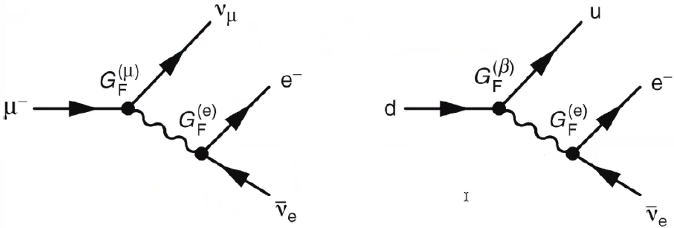
\includegraphics[width=0.6\textwidth]{meson_mixing_and_oscillations/verval_mu_d.png}
        \label{fig:meson_mixing_and_oscillations/verval_mu_d}
    }\\
    \subfloat[Verval van pion en kaon]{
        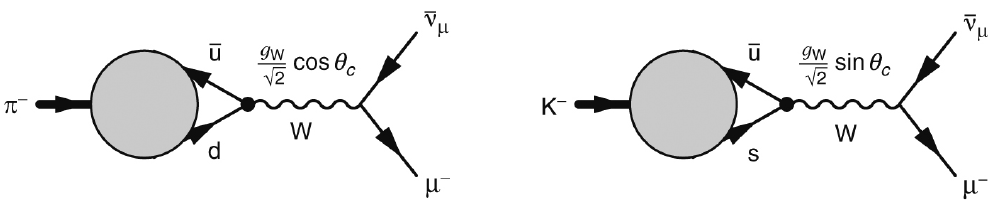
\includegraphics[width=0.8\textwidth]{meson_mixing_and_oscillations/verval_pi_k.png}
        \label{fig:meson_mixing_and_oscillations/verval_pi_k}
    }
    \caption{Feynman diagrammen van zwakke quark mixing}
\end{figure}

De onderdrukking van het kaon kan hieruit makkelijk getoond worden omdat met $\theta_c \approx 12^\circ$ de sinus veel kleiner zal zijn dan de cosinus.

\subsection{Cabbibo theorie}%
\label{sub:cabbibo_theorie}

Deze theorie was niet zonder zijn fouten. Dit geeft aanleiding tot het zogenaamde flavour changing neutral current probleem.

\begin{figure}[h]
    \centering
    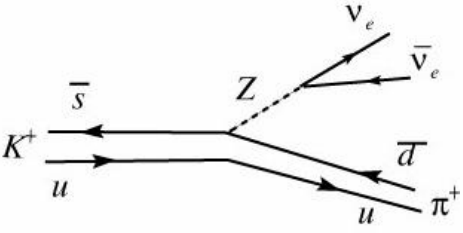
\includegraphics[width=0.5\linewidth]{meson_mixing_and_oscillations/flav_ch_problem.png}
    \caption{Voorbeeld van het flavour changing neutral current probleem}%
    \label{fig:meson_mixing_and_oscillations/flav_ch_problem}
\end{figure}

Dit verval is nog nooit waargenomen. Dit verranderen van kleur met behulp van een $Z$ boson is enkel mogelijk als $s$ via $s'$ kan vervallen naar $d$.

\subsection{GIM-mechanisme}%
\label{sub:gim_mechanisme}

Het is maar een paar jaar later dat de $s$ quark samen met de $c$ quark in een doublet worden samengebracht. Dit zorgt voor extra termen in de Lagrangiaan die elkaar opheffen in alle ordes.

\begin{figure}[h]
    \centering
    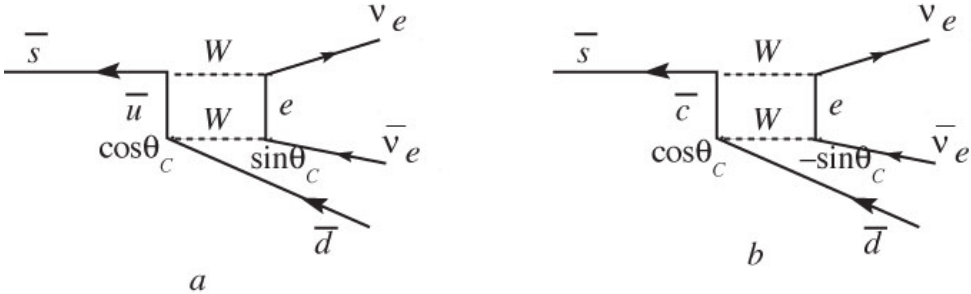
\includegraphics[width=0.6\linewidth]{meson_mixing_and_oscillations/gim_opheffing.png}
    \caption{Opheffing van de opmengende termen in de GIM theorie}%
    \label{fig:meson_mixing_and_oscillations/gim_opheffing}
\end{figure}

We gaan hier niet verder in op de uitwerking van de Lagrangiaan. Uit dit GIM-mechanisme komt wel dat de er nu geen Flavour Changing Neutral Currents meer zijn. De prijs die we hiervoor moeten bestalen is de toevoeging van de $c$ quark die in 1974 dan ook is ontdekt ($J/\Psi$).

\subsection{Meer FCNC}%
\label{sub:meer_fcnc}

\begin{figure}[h]
    \centering
    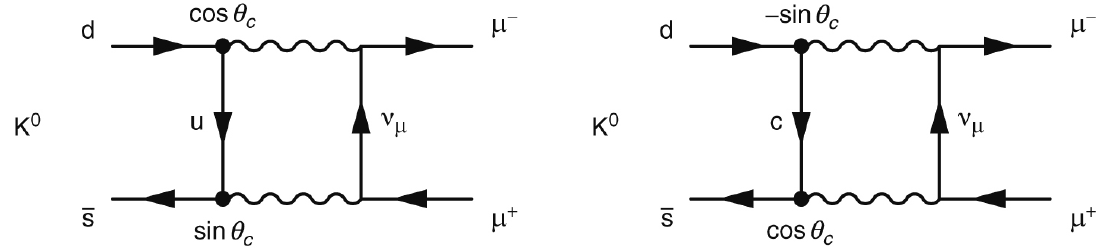
\includegraphics[width=0.8\linewidth]{meson_mixing_and_oscillations/fcnc.png}
    \caption{Box diagrammen voor kaon verval naar muonen}%
    \label{fig:meson_mixing_and_oscillations/fcnc}
\end{figure}

Indien we enkel de Cabbibo theorie zouden hebben is enkel het eerste diagram mogelijk en zouden de waarschijnlijkheden veel te groot zijnom de vervallen (branching fraction is te groot). In de GIM theorie zullen de 2 diagrammen met $u$ en $c$ elkaar uitcancelen.
\begin{equation}
    \begin{aligned}
        \label{eq:fcnc_mat_el}
        \mathcal{M}_{u} &\propto g_{W}^{4} \cos \theta_{C} \sin \theta_{C}\\
        \mathcal{M}_{c} &\propto-g_{W}^{4} \cos \theta_{C} \sin \theta_{C}\\
        |\mathcal{M}|^{2}&=\left|\mathcal{M}_{u}+\mathcal{M}_{c}\right|^{2} \approx 0
    \end{aligned}
\end{equation}
Het totaal matrix element zal niet volledig 0 zijn omdat de massa's van $c$ en $u$ niet volledig hetzelfde zijn. De massa van $c$ is groter en dus minder waarschijnlijk. In combinatie met de experimentele resultaten van de branching fraction van deze vervallen was het mogelijk om de massa van de $c$ quark te voorspellen.

\subsection{CKM matrix}%
\label{sub:ckm_matrix}

In 1979 was er dan in tegenstelling van het ontdekken van het $c$ quark een ``echte'' revolutie in de deeltjes fysica. De ontdekking van de derde generatie quarks is gebeurd.
\begin{equation}
    \begin{aligned}
        \label{eq:ckm_mat}
        \left(\begin{array}{c}
                d^{\prime} \\
                s^{\prime} \\
                b^{\prime}
                \end{array}\right)=V_{C K M}\left(\begin{array}{l}
                d \\
                s \\
                b
        \end{array}\right)
    \end{aligned}
\end{equation}
Dit moet een unitaire matrix zijn omdat 1 quark in de ene toestand nog steeds 1 quark moet zijn in de andere. Dit is gegeven door het behoud van waarschijnlijkheid. Dit is in het geval dat er maar 3 quarks mixen wat we natuurlijk willen testen. Een unitaire matrix van dimensie $N$ heeft $(N-1)^2$ vrijheidsgraden. Deze zijn de 3 euler hoeken en een fase.\\
Deze matrix kan op verschillende manieren geparametriseerd worden. Een eerste mogelijkheid is aan de hand van de CC interacties
\begin{equation}
    \begin{aligned}
        \label{eq:cc_int_ckm}
        \left(\begin{array}{ccc}
                \bar{u} & \bar{c} & \bar{t}
                \end{array}\right) \hat{O}_{C C}^{\mu}\left(\begin{array}{ccc}
                V_{u d} & V_{u s} & V_{u b} \\
                V_{c d} & V_{c s} & V_{c b} \\
                V_{t d} & V_{t s} & V_{t b}
                \end{array}\right)\left(\begin{array}{l}
                d^{\prime} \\
                s^{\prime} \\
                b^{\prime}
        \end{array}\right)
    \end{aligned}
\end{equation}
Origineel zag die er niet zo uit.
\begin{equation}
    \begin{aligned}
        \label{eq:ckm_origineel}
        \left(\begin{array}{ccc}
                c_{1} & -s_{1} c_{3} & -s_{1} s_{3} \\
                s_{1} c_{2} & c_{1} c_{2} c_{3}-s_{2} s_{3} e^{i \delta} & c_{1} c_{2} s_{3}+s_{2} c_{3} e^{i \delta} \\
                s_{1} s_{2} & c_{1} s_{2} c_{3}+c_{2} s_{3} e^{i \delta} & c_{1} s_{2} s_{3}-c_{2} c_{3} e^{i \delta}
        \end{array}\right)
    \end{aligned}
\end{equation}
Hierbij is $c_1 = \cos\theta_1$ de cos van de Cabbibo hoek en $s_1 = \sin\theta_1$ de sin van de Cabbibo hoek. De indexen refereren naar de generatie. Dit kan nog uitgebreid worden naar:
\begin{equation}
    \begin{aligned}
        \label{eq:ckm_uitgebreid}
        \left(\begin{array}{ccc}
                c_{12} c_{13} & s_{12} c_{13} & s_{13} e^{-i \delta_{13}} \\
                -s_{12} c_{23}-c_{12} s_{23} s_{13} e^{i \delta_{13}} & c_{12} c_{23}-s_{12} s_{23} s_{13} e^{i \delta_{13}} & s_{23} c_{13} \\
                s_{12} s_{23}-c_{12} c_{23} s_{13} e^{i \delta_{13}} & -c_{12} s_{23}-s_{12} c_{23} s_{13} e^{i \delta_{13}} & c_{23} c_{13}
        \end{array}\right)
    \end{aligned}
\end{equation}
Ten laatste hebben we nog een alternatieve notatie met als naam Wolfenstein.
\begin{equation}
    \begin{aligned}
        \label{eq:wolfenstein_ckm}
        \left(\begin{array}{ccc}
                1-\lambda^{2} / 2 & \lambda & A \lambda^{3}(\rho-i \eta) \\
                -\lambda & 1-\lambda^{2} / 2 & A \lambda^{2} \\
                A \lambda^{3}(1-\rho-i \eta) & -A \lambda^{2} & 1
        \end{array}\right)+O\left(\lambda^{4}\right)
    \end{aligned}
\end{equation}
Focussen we eerst op de uitgebreide CKM-matrix uit vergelijking (\ref{eq:ckm_uitgebreid}). Deze kunnen we herschrijven in 3 aparte matrixen.
\begin{equation}
    \begin{aligned}
        \label{eq:ckm_uitgebreid_split}
        V_{C K M}=&\left(\begin{array}{ccc}
                1 & 0 & 0 \\
                0 & c_{23} & s_{23} \\
                0 & -s_{23} & c_{23}
            \end{array}\right) \times\left(\begin{array}{ccc}
                c_{13} & 0 & s_{13} e^{-i \delta} \\
                0 & 1 & 0 \\
                -s_{13} e^{i \delta} & 0 & c_{13}
            \end{array}\right) \\
            & \times\left(\begin{array}{ccc}
                c_{12} & s_{12} & 0 \\
                -s_{12} & c_{12} & 0 \\
                0 & 0 & 1
        \end{array}\right)
    \end{aligned}
\end{equation}
Het is zoals eerder gezegd mogelijk om deze matrix te beschijven als we de eulerhoeken $\theta_1$, $\theta_2$, $\theta_3$ en de fase $\delta$. De relatie tussen de verschillende vormen zijn makkelijk uit te rekenen.
\begin{equation}
    \begin{aligned}
        \label{eq:ckm_relaties}
        s_{12} &=\lambda=\frac{\left|V_{u s}\right|}{\sqrt{\left|V_{u s}\right|^{2}+\left|V_{u d}\right|^{2}}} \\
        s_{23} &=A \lambda^{2}=\lambda\left|\frac{V_{c b}}{V_{u s}}\right| \\
        s_{13} e^{i \delta} &=V_{u b}^{*}=A \lambda^{3}(\rho+i \eta)
    \end{aligned}
\end{equation}

\subsection{CKM matrix elementen}%
\label{sub:ckm_matrix_elementen}

Hoe bepalen we deze elementen nu? Eerst moeten we met hoge precisie bepalen we de zwakke koppelingsconstante $G_F$ is. Dit kunnen we doen door het onderzoek van het zwakke verval van leptonen.

\begin{figure}[h]
    \centering
    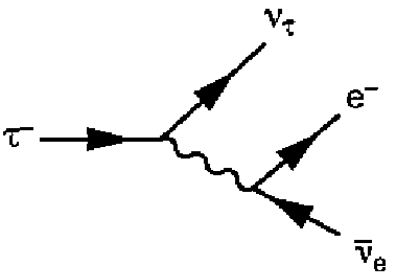
\includegraphics[width=0.5\linewidth]{meson_mixing_and_oscillations/zwak_lep_verval.png}
    \caption{Feynman diagram van lepton verval}%
    \label{fig:meson_mixing_and_oscillations/zwak_lep_verval}
\end{figure}

\begin{equation}
    \begin{aligned}
        \label{eq:lep_verval_zwak}
        \Gamma\left(\mu^{-} \rightarrow \nu_{\mu} e^{-} \bar{\nu}_{e}\right) &=\frac{G_{F}^{2} m_{\mu}^{5}}{192 \pi^{3}}\left(1+\delta_{e}^{\mu}\right) \\
        \Gamma\left(\tau^{-} \rightarrow \nu_{\tau} e^{-} \bar{\nu}_{e}\right) &=\frac{G_{F}^{2} m_{\tau}^{5}}{192 \pi^{3}}\left(1+\delta_{e}^{\tau}\right) \\
                                                                               &=\frac{B\left(\tau^{-} \rightarrow \nu_{\tau} e^{-} \bar{\nu}_{e}\right)}{\tau_{\tau}}
    \end{aligned}
\end{equation}
Wat zien in deze vergelijkingen is de waarschijnlijkheid dat het lepton vervalt in zijn neutrino, een elektron en een antineutrino. In deze waarschijnlijkheid hebben we een $G_F$ in het kwadraat omdat er 2 vertexes zijn aan het $W$ boson. Dit is zuiver leptonisch dus komen hier geen Cabbibo hoeken aan te pas. De reden voor de massa tot de 5de term is het gevolg van het vervallen van 1 deeltje in 3. Dit geeft ons 2 vrijheidsgraden dit geeft ons een $p^2p^2dp$ wat ons $E^5$ geeft. De enige energie vrijheidsgraad dat we hebben is de massa van ons initieel deeltje dus hebben we een $m^5$ term. $\delta$ is een correctie term voor al de fysica die we hier niet in acht hebben genomen zoals de massa van het elektron, de radiatieve correcties... We moeten hier natuurlijk opletten dat we niet naar de totale breedte van de leptonen kijken maar eerder naar de branching fractie $B(...)$ naar specifiek het verval aan de hand van een $W^-$ boson in verhouding tot de levensduur van het lepton. Nu we weten wat $G_F$ is kunnen we overgaan naar zwakke vervallen van de quarks in mesonen die wel een Cabbibo hoek bevatten.

\begin{figure}[h]
    \centering
    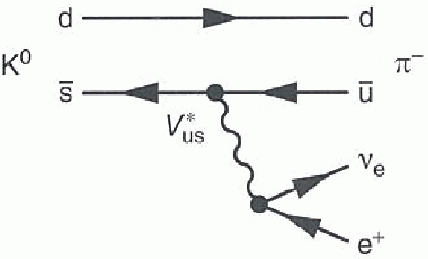
\includegraphics[width=0.5\linewidth]{meson_mixing_and_oscillations/zwak_s_verval.png}
    \caption{Feynman diagram van het zwak kaon verval}%
    \label{fig:meson_mixing_and_oscillations/zwak_s_verval}
\end{figure}

\begin{equation}
    \begin{aligned}
        \label{eq:kaon_zwak_verval}
        Gamma\left(K^{0} \rightarrow \pi^{-} e^{+} \nu_{e}\right) &=\frac{G_{F}^{2} m_{K}^{5}}{192 \pi^{3}}\left(1+\delta_{e}^{K}\right)\left|V_{u s}\right|^{2} \\
                                                                  &=\frac{B\left(K^{0} \rightarrow \pi^{-} e^{+} \nu_{e}\right)}{\tau_{K}}
    \end{aligned}
\end{equation}
De vertex voor het verval van $W^+$ naar het positron en de neutrino is niets anders dan $G_F$. Voor de koppeling van $W$ aan de quarks hebben we naast $G_F$ nog een extra term $|V_{us}|^2$ met het kwadraat omdat dit een waarschijnlijkheid moet zijn. $d$ is hier alleen een bijstaander en als deze iets zou bijgeven aan deze vergelijking is het verwerkt in de correctieterm $\delta$. Uit de experimenten is het dus mogelijk om $|V_{us}|$ te bepalen en niet $V_{us}$. We krijgen $\left|V_{us}\right|=0.2252(9)$.\\
Hetzelfde kan gedaan worden voor $B$ mesonen.

\begin{figure}[h]
    \centering
    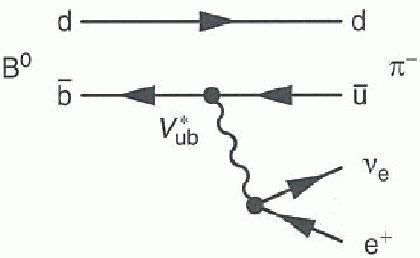
\includegraphics[width=0.5\linewidth]{meson_mixing_and_oscillations/zwak_b_verval.png}
    \caption{Feynman diagram van het zwak kaon verval}%
    \label{fig:meson_mixing_and_oscillations/zwak_b_verval}
\end{figure}

\begin{equation}
    \begin{aligned}
        \label{eq:b_zwak_verval}
        \Gamma\left(B^{0} \rightarrow \pi^{-} e^{+} \nu_{e}\right) &=\frac{G_{F}^{2} m_{B}^{5}}{192 \pi^{3}}\left(1+\delta_{e}^{B}\right)\left|V_{u b}\right|^{2} \\
                                                                   &=\frac{B\left(B^{0} \rightarrow \pi^{-} e^{+} \nu_{e}\right)}{\tau_{B}}
    \end{aligned}
\end{equation}
We vinden nu dat $\left|V_{u b}\right|=(4.15 \pm 0.49) \times 10^{-3}$ is.\newpage
Uit het verschil tussen $\left|V_{us}\right| > \left|V_{u b}\right|$ kunne we direct inzien dat het verval via $W^+$ naar een pion veel onwaarschijnlijker is voor het $B$ meson dan voor het $K$ meson.\\
Zo is het mogelijk om voor alle andere CKM-matrix elementen deze ook experimenteel te bepalen:
\begin{itemize}
    \item Superallowed nucleaire $\beta$ verval $\Rightarrow\left|V_{u d}\right|=0.97425(22)$
    \item $D^{\pm} \rightarrow \pi^{0} l^{\pm} \nu_{l} \Rightarrow\left|V_{c d}\right|=0.230(11)$\\
        \begin{center}
            \begin{tikzpicture}
                \begin{feynman}
                    \vertex (b1) {\(\overline c\)};
                    \vertex[right=2cm of b1] (b2) node [above=0.1em of b2] {\(V_{cd}^*\)};
                    \vertex[right=2cm of b2] (b3) {\(\overline d\)};

                    \vertex[above=2em of b1] (a1) {\(d\)};
                    \vertex[above=2em of b3] (a2) {\(d\)};

                    \vertex[below=2em of b3] (c1) {\(e^+\)};
                    \vertex[below=2em of c1] (c2) {\(\overline \nu_e\)};
                    \vertex at ($(c1)!0.5!(c2) - (1cm, 0)$) (d);
                    \diagram* {
                        (a1) -- [fermion] (a2),
                        (b3) -- [fermion] (b2) -- [fermion] (b1),
                        (c2) -- [fermion, out=180, in=-45] (d),
                        (c1) -- [fermion, out=180, in=45] (d),
                        (b2) -- [boson, bend right, edge label=\(W^{+}\)] (d),
                    };
                    \draw [decoration={brace}, decorate] (b1.south west) -- (a1.north west)
                    node [pos=0.5, left] {\(D^{-}\)};
                    \draw [decoration={brace}, decorate] (a2.north east) -- (b3.south east)
                    node [pos=0.5, right] {\(\pi^{0}\)};
                \end{feynman}
            \end{tikzpicture}
        \end{center}
    \item $D_{s}^{+} \rightarrow \mu^{+} \nu_{\mu} \Rightarrow\left|V_{c s}\right|=1.006 \pm 0.023$
        \begin{center}
            \begin{tikzpicture}
                \begin{feynman}
                    \vertex (i1) {\(c\)};
                    \vertex[below=4em of i1] (i2) {\(\overline s\)};
                    
                    \vertex[right=3cm of i1] (f1) {\(\mu^+\)};
                    \vertex[below=4em of f1] (f2) {\(\nu_\mu\)};

                    \vertex at ($(i1)!0.5!(i2) + (1cm, 0)$) (a) node [above=0.1em of a] {\(V_{cs}^*\)};
                    \vertex at ($(f1)!0.5!(f2) - (1cm, 0)$) (b);

                    \diagram* {
                        (i1) -- [fermion] (a) -- [fermion] (i2),
                        (f2) -- [fermion] (b) -- [fermion] (f1),
                        (a) -- [boson, edge label=\(W^{+}\)] (b),
                    };
                    \draw [decoration={brace}, decorate] (i2.south west) -- (i1.north west)
                    node [pos=0.5, left] {\(D^{+}_s\)};
                \end{feynman}
            \end{tikzpicture}
        \end{center}
    \item $b \rightarrow l \nu c \Rightarrow\left|V_{c b}\right|=(40.9 \pm 1.1) \times 10^{-3}$
        \begin{center}
            \begin{tikzpicture}
                \begin{feynman}
                    \vertex (b1) {\(\overline b\)};
                    \vertex[right=2cm of b1] (b2) node [above=0.1em of b2] {\(V_{cb}^*\)};
                    \vertex[right=2cm of b2] (b3) {\(\overline c\)};

                    \vertex[above=2em of b1] (a1) {\(u\)};
                    \vertex[above=2em of b3] (a2) {\(u\)};

                    \vertex[below=2em of b3] (c1) {\(e^+\)};
                    \vertex[below=2em of c1] (c2) {\(\overline \nu_e\)};
                    \vertex at ($(c1)!0.5!(c2) - (1cm, 0)$) (d);
                    \diagram* {
                        (a1) -- [fermion] (a2),
                        (b3) -- [fermion] (b2) -- [fermion] (b1),
                        (c2) -- [fermion, out=180, in=-45] (d),
                        (c1) -- [fermion, out=180, in=45] (d),
                        (b2) -- [boson, bend right, edge label=\(W^{+}\)] (d),
                    };
                    \draw [decoration={brace}, decorate] (b1.south west) -- (a1.north west)
                    node [pos=0.5, left] {\(B^{+}\)};
                    \draw [decoration={brace}, decorate] (a2.north east) -- (b3.south east)
                    node [pos=0.5, right] {\(D^{0}\)};
                \end{feynman}
            \end{tikzpicture}
        \end{center}
\end{itemize}
Het is uiteindelijk mogelijk om op verschillende manieren deze koppelingen te bepalen en zien dat deze altijd binnen elkaars fout vallen.\\
De laatste overgebleven matrix elementen moeten we halen uit de box diagrammen van de meson oscillaties:
\begin{itemize}
    \item $B^0$ oscillaties: $\left|V_{t d}\right|=(8.4 \pm 0.6) \times 10^{-3}$
    \item $B_S^0$ oscillaties: $\left|V_{t s}\right|=(42.9 \pm 2.6) \times 10^{-3}$
\end{itemize}
{\color{blue} Intermezzo: Wat zijn de quark combinaties van de mesonen?\\
    $K$ mesonen bestaan uit een $s$ quark met een andere quark:
    \begin{equation}
        \begin{aligned}
            \label{eq:k_meson_samenstelling}
            K^+ &= \left| u\bar{s}\right>\\
            K^- &= \left| \bar{u}s\right>\\
            K^0 &= \left| d\bar{s}\right>\\
            \bar{K}^0 &= \left| \bar{d}s\right>\\
        \end{aligned}
    \end{equation}
    $D$ mesonen bestaan uit een $c$ quark met een andere quark:
    \begin{equation}
        \begin{aligned}
            \label{eq:d_meson_samenstelling}
            D^+ &= \left| c\bar{d}\right>\\
            D^- &= \left| \bar{c}d\right>\\
            D^0 &= \left| c\bar{u}\right>\\
            \bar{D}^0 &= \left| \bar{c}u\right>\\
        \end{aligned}
    \end{equation}
    $B$ mesonen bestaan uit een $b$ quark met een andere quark:
    \begin{equation}
        \begin{aligned}
            \label{eq:d_meson_samenstelling}
            B^+ &= \left| u\bar{b}\right>\\
            B^- &= \left| \bar{b}b\right>\\
            B^0 &= \left| d\bar{b}\right>\\
            B_S &= \left| s\bar{b}\right>\\
        \end{aligned}
    \end{equation}
    Er wordt op het examen echt wel verwacht dat je dit kan.
}

\subsection{Unitariteit van de CKM-matrix}%
\label{sub:unitariteit_van_de_ckm_matrix}

Vanwege het behoud van waarschijnlijkheid moet de matrix unitair zijn. De sommaties van de kwadraten van de elementen in een rij of kolem moeten dus gelijk zijn aan 1. Dit nemen we ook waar:
\begin{itemize}
    \item 1ste rij: $\left|V_{u d}\right|^{2}+\left|V_{u s}\right|^{2}+\left|V_{u b}\right|^{2}=0.9999(6)$
    \item 2de rij: $\left|V_{c d}\right|^{2}+\left|V_{c s}\right|^{2}+\left|V_{c b}\right|^{2}=1.067(47)$
    \item 1ste kolom: $\left|V_{u d}\right|^{2}+\left|V_{c d}\right|^{2}+\left|V_{t d}\right|^{2}=1.002(5)$
    \item 2de kolom: $\left|V_{u s}\right|^{2}+\left|V_{c s}\right|^{2}+\left|V_{t s}\right|^{2}=1.065(46)$
\end{itemize}
Tot op eerste orde kunnen we dus zien dat de unitariteit is behouden. Indien er dus nog een 4de generatie aan quarks zou bestaan mag deze niet koppelen met de eerste 3 generaties. fitten we de matrix elementen nu aan deze uitkomsten en doordat deze unitair moet zijn krijgen we een CKM-matrix die er als volgt uit ziet:
\begin{equation}
    \begin{aligned}
        \label{eq:ckm_huidig}
        \left(\begin{array}{ccc}
                \left|V_{u d}\right| & \left|V_{u s}\right| & \left|V_{u b}\right| \\
                \left|V_{c d}\right| & \left|V_{c s}\right| & \left|V_{c b}\right| \\
                \left|V_{t d}\right| & \left|V_{t s}\right| & \left|V_{t b}\right|
                \end{array}\right) \approx\left(\begin{array}{ccc}
                0.974 & 0.225 & 0.004 \\
                0.225 & 0.973 & 0.041 \\
                0.009 & 0.040 & 0.999
        \end{array}\right)
    \end{aligned}
\end{equation}
Het is duidelijk te zien met de diagonaal elementen die zo goed als 1 zijn dat we vooral binnen de generatie zelf blijven. De koppeling tussen de eerste en 2de generatie is vrij groot, dit is de Cabbibo hoek $\theta_{12} = 12.9^\circ$. De koppeling tussen de 2de en 3de generatie is een stuk kleiner met een koppelingshoek $\theta_{23} = 2.4^\circ$. En ten laatste koppelt de eerste en 3de generatie zo goed als niet ($\theta_{13} = 0.2^\circ$).

\end{document}
